\documentclass[letterpaper]{article}
\usepackage[submission]{aaai2026}
\usepackage{times}
\usepackage{helvet}
\usepackage{courier}
\renewcommand{\ttdefault}{cmtt}
\usepackage[hyphens]{url}
\usepackage{graphicx}
\urlstyle{rm}
\def\UrlFont{\rm}
\usepackage{natbib}
\usepackage{caption}
\usepackage{amsmath,amssymb,amsthm}
\usepackage{booktabs}
\usepackage{algorithm}
\usepackage{algpseudocode}
\frenchspacing
\setlength{\pdfpagewidth}{8.5in}
\setlength{\pdfpageheight}{11in}
\pdfinfo{
/TemplateVersion (2026.1)
}

\newcommand{\WMC}{\ensuremath{\mathrm{WMC}}}
\newcommand{\tw}{\ensuremath{\mathrm{tw}}}
\newcommand{\R}{\mathbb{R}}
\newcommand{\bC}[1]{\boldsymbol{#1}}
\newtheorem{theorem}{Theorem}
\newtheorem{definition}{Definition}
\newtheorem{proposition}{Proposition}
\newtheorem{example}{Example}

\title{Technical Supplement: Scaling Ontology-Conditioned Weighted Model Counting with Modular Separators}
\author{
    Anonymous Submission
}
\affiliations{
    Anonymous Institution\\
}
\newcommand{\stitle}[1]{\vspace{1mm}\noindent\textit{#1}}

\begin{document}
\maketitle

\begin{abstract}
This supplement provides additional theory and diagnostics, full
reproducibility and optimization details, ontology instantiation protocols,
a Lean formalization inventory, and extended neuro-symbolic comparisons for
the accompanying paper.
\end{abstract}

\appendix
\section{Ethical Statement}
This work uses publicly available ontologies (GO, UBERON, ChEBI) and poses no human-subjects risk. Improved ontology consistency may affect automated annotation quality. The marginals $\mu_i$ provide a structural correction layer; clinical prediction requires independent validation and additional evidence.

\section{Reproducibility Details}
\label{app:reproducibility}

\paragraph{Experiment protocol.}
The operational selector uses the boundary-aware core-selection algorithm in the main paper with
\(w_{\max}=14\), \(\beta=0.01\), and \(\rho=0.30\); reported widths are
min-fill upper bounds. Direct TT fitting uses
\(r\in\{1,2,4,8\}\), 5,000 unique training queries for complete-ontology
runs, six alternating-least-squares sweeps, nonnegative least-squares core
updates, and an independent validation set. Scores used by the TT path are
clipped to \([10^{-6},1-10^{-6}]\). Loopy BP uses synchronous sum-product
updates with damping \(0.5\), tolerance \(10^{-9}\), and at most 20,000
iterations. Exact-reference candidates use 108 retained subgraphs from
each of GO mf, GO bp, UBERON, and ChEBI; every retained instance has
agreeing brute-force and junction-tree references under fixed random seeds.

\paragraph{Compute resources.}
The ontology experiments are CPU-only SLURM runs. Multi-ontology screening
uses 16 CPU cores and 128\,GB allocated memory. The full ChEBI recursive
run uses one CPU core and 400\,GB allocated memory. Monolithic JT rows use
a common 300\,GB memory cap. Downstream GO cc exact-WMC post-processing uses
the same junction-tree backend as the intrinsic GO cc reference run.

\paragraph{Data availability.}
The anonymized submission artifact contains source code, ontology
preprocessing, exact and approximate inference backends, Lean developments,
environment files, seeds, raw results, and table-generation scripts. Every
reported row is generated from a versioned configuration in that artifact.

\paragraph{Direct TT optimization.}
\label{app:direct-tt-optimization}
For each direct TT separator, boundary assignments are sampled uniformly
without replacement and logically supported assignments form the training
set. Positive oracle targets are scaled by their maximum. The fit uses six
alternating-least-squares sweeps; each binary core slice is updated by
nonnegative least squares from a positive random initialization. The
relative ridge starts at \(10^{-4}\) and increases through
\(\{10^{-2},10^{-1},1\}\) when the linear solve is singular. A disjoint
uniform validation set reports normalized MAE.

\section{Additional Theory and Diagnostics}
\label{app:additional-theory}

\paragraph{General Boolean queries.}
For any Boolean query \(\psi\), the ontology-conditioned probability is
\[
p_T(\psi)
=
\frac{\mathrm{WMC}(T\wedge \psi,p)}
     {\mathrm{WMC}(T,p)}.
\]

\paragraph{Local exactness on a star.}
Consider a parent concept \(\pi\) with children \(c_1,\ldots,c_k\) and
constraints \(y_{c_j}\Rightarrow y_\pi\). Let \(p_\pi\) be the score of
the parent, and let \(m_1,\ldots,m_k\) be incoming child messages. The
local true-path update is
\[
S_\pi(m_1,\ldots,m_k)
=
\frac{p_\pi}
     {p_\pi+(1-p_\pi)\prod_{j=1}^{k}(1-m_j)}.
\]

\begin{theorem}[Star exactness]
\label{thm:star}
For a parent \(\pi\) with independent children
\(c_1,\ldots,c_k\) under the constraints
\(y_{c_j}\Rightarrow y_\pi\), the exact WMC marginal of \(y_\pi\) is
\[
\mu_\pi
=
\frac{p_\pi}
     {p_\pi+(1-p_\pi)\prod_{j=1}^{k}(1-p_{c_j})}.
\]
\end{theorem}

The result follows by conditioning on \(y_\pi\): all child assignments
are allowed when \(y_\pi=1\), whereas every child must be false when
\(y_\pi=0\).

\paragraph{Diamond calculation.}
\label{app:diamond-calculation}
For the diamond \(T_{\diamond}\) in the reconvergent-diamond discussion in the main paper
with all four Bernoulli parameters equal to \(1/2\), six assignments
satisfy the implications. Five of those assignments have \(y_a=1\), giving
\(p_{T_{\diamond}}(y_a=1)=5/6\). The path-wise calculation first sends
the evidence from \(d\) to the two intermediate variables,
\[
m_b=m_c
=
\frac{1/2}{1/2+(1/2)(1-1/2)}
=
\frac{2}{3},
\]
and then combines the two incoming messages at \(a\),
\[
\widehat{\mu}_a
=
\frac{1/2}{1/2+(1/2)(1-2/3)^2}
=
\frac{9}{10}.
\]

\paragraph{Dense-mode computational scope.}
\label{app:dense-cost}
Let \(n_j=|M_j|\), let \(\widehat w_j^\partial\) be the boundary-last
module width, and let \(\widehat w_C\) be the induced width of the reduced
core. Exact dense-mode elimination costs, up to backend constants,
\[
O\!\left(
\sum_{j=1}^{s}\!\left[n_j2^{\widehat w_j^\partial+1}+2^{|B_j|}\right]
+
(|C|+s)2^{\widehat w_C+1}
\right).
\]

\paragraph{Proof of the module-recovery stability proposition.}
\label{app:boundary-error-proof}
Module recovery applies the same Markov kernel
\(K_j(y_{M_j}\mid y_{B_j})\) to the exact and approximate boundary
posteriors. Total variation distance contracts under a Markov kernel,
which yields the stated inequality.

\paragraph{Reconvergence diagnostic.}
Table~\ref{tab:reconv} evaluates local propagation on fragments with and
without shared-evidence reconvergence.

\begin{table}[t]
\centering
\small
\setlength{\tabcolsep}{3pt}
\begin{tabular}{ll}
\toprule
Case & Result \\
\midrule
Single edge & error \(\le 5{\times}10^{-13}\) \\
Three-child star & error \(\le 5{\times}10^{-13}\) \\
Two-parent polytree & agrees with WMC \\
Diamond, path-wise & \(5/6\) vs. \(9/10\) \\
Diamond, loopy BP & max diff. \(5.8{\times}10^{-2}\) \\
GO cc, loopy BP & MAE \(2.1{\times}10^{-4}\) \\
GO cc, loopy BP & max error \(6.4{\times}10^{-2}\) \\
GO cc, loopy BP & \(0.6\%\) above \(10^{-2}\) \\
GO cc multi-parent & \(6.0{\times}\) larger error \\
Extreme GO mf, loopy BP & \(0.16\%\) violations \\
\bottomrule
\end{tabular}
\caption{Reconvergence diagnostic. The elementary cases isolate when
local updates agree with WMC and when reconvergent evidence reuse changes
the target.}
\label{tab:reconv}
\end{table}

Across score families, exact inference remains coherent, whereas loopy
BP can converge while still changing the target and producing violations
under extreme scores. On GO bp, exact inference provides the stable
reference used to quantify the slower convergence profile of loopy BP.

\paragraph{Core-selection ablation.}
Table~\ref{tab:core-ablation} compares core selectors at a matched
variable budget. The result shows that the reported
min-fill-contribution selector delivers the narrowest augmented modules
among these selectors, so the selector ranking contributes directly to
decomposition quality.

\begin{table}[t]
\centering
\small
\setlength{\tabcolsep}{3pt}
\begin{tabular}{lc}
\toprule
Selector & Unrestricted \(\max_j\widehat w(A_j)\) \\
\midrule
Boundary-aware & 6 \\
Residual-width & 6 \\
Min-fill contribution & \textbf{5} \\
Static degree & 10 \\
Dynamic degree & 11 \\
Random (10 seeds) & 12 (infeasible) \\
\bottomrule
\end{tabular}
\caption{Core-selection ablation on GO cc at a matched 40-atom core
budget. Structured selectors produce exactly solvable modules at this
budget.}
\label{tab:core-ablation}
\end{table}

\section{Auxiliary Inference Results}

\paragraph{Unrestricted structural pre-screen.}
Table~\ref{tab:structure-decomposition} reports the decomposition
diagnostic based on unrestricted augmented-module width. It measures the
structural premise that a small core can isolate most ontology variables
in substantially narrower components. The operational boundary-last
measure used by the boundary-aware core-selection algorithm in the main paper is reported in
the main ontology-scale experiment.

\begin{table*}[t]
\centering
\small
\setlength{\tabcolsep}{5pt}
\begin{tabular}{lrrrrrrrr}
\toprule
Ontology & Terms & \%mp & Max deg. & \(\widehat w(G_T)\)
& Core & Modules & \(\max_j\widehat w(A_j)\) & Struct. cov. \\
\midrule
GO cc  & 4,041   & 13.0 & 4  & 12  & 0.0\% & 1       & 12 & 100.0\% \\
GO mf  & 10,131  & 20.0 & 7  & 37  & 5.0\% & 6,519   & 5  & 95.0\%  \\
GO bp  & 25,950  & 53.0 & 9  & 269 & 9.0\% & 7,249   & 12 & 91.0\%  \\
UBERON & 14,977  & 24.0 & 7  & 46  & 5.0\% & 8,427   & 11 & 95.0\%  \\
ChEBI  & 205,592 & 24.7 & 14 & 738 & 2.0\% & 181,679 & 12 & 98.0\%  \\
\bottomrule
\end{tabular}
\caption{Unrestricted modular pre-screen. Structural coverage is
\(\sum_j|M_j|/|Y|=1-|C|/|Y|\).}
\label{tab:structure-decomposition}
\end{table*}

\paragraph{GO cc inference baselines.}
Table~\ref{tab:go-cc-baselines} retains the complete same-semantics
baseline measurements. The forced modular configuration exercises
separator construction and recovery; the automatic policy uses the
monolithic exact backend when the whole graph already meets the width cap.

\begin{table}[t]
\centering
\scriptsize
\setlength{\tabcolsep}{3pt}
\begin{tabular}{lrrr}
\toprule
Method & MAE & Max error & Time \\
\midrule
Exact JT & Ref. & Ref. & 2.42s \\
Loopy BP & \(2.05{\times}10^{-4}\) & \(6.4{\times}10^{-2}\) & 0.065s \\
Mini-bucket, \(i{=}8\) & \(5.60{\times}10^{-4}\) & \(2.36{\times}10^{-1}\) & 1.19s \\
Mini-bucket, \(i{=}12\) & \(2.97{\times}10^{-19}\) & \(1.11{\times}10^{-16}\) & 1.18s \\
Ours, forced exact factors & \(1.95{\times}10^{-17}\) & \(3.33{\times}10^{-16}\) & 51.4s \\
PySDD & -- & -- & OOM \\
\bottomrule
\end{tabular}
\caption{Full GO cc diagnostic. PySDD exhausted 32, 96, and 256\,GB
memory caps.}
\label{tab:go-cc-baselines}
\end{table}

\paragraph{Dense-separator representation diagnostic.}
Figure~\ref{fig:width-rank-appendix} and Table~\ref{tab:separator-rank}
provide additional dense-table diagnostics. They measure compressibility
after exact enumeration and complement the direct-TT end-to-end evidence in
the main experiments.

\begin{figure}[t]
\centering
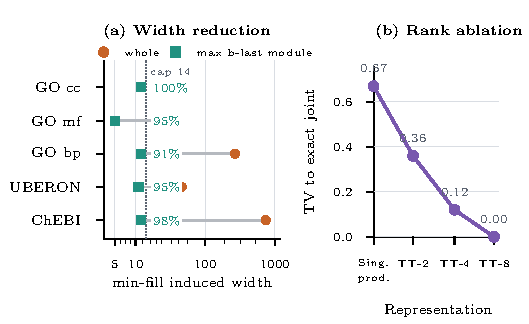
\includegraphics[width=\columnwidth]{fig_width_rank.pdf}
\caption{Structural and representation diagnostics. (a)
Unrestricted min-fill width before and after the structural pre-screen.
(b) TT-SVD representation error on one exactly enumerated 10-variable GO
cc separator.}
\label{fig:width-rank-appendix}
\end{figure}

\begin{table}[t]
\centering
\small
\setlength{\tabcolsep}{6pt}
\begin{tabular}{lrr}
\toprule
Ontology & Product TV & Product MAE \\
\midrule
GO cc  & 0.0215 & \(6.96{\times}10^{-3}\) \\
GO mf  & 0.0000 & \(3.85{\times}10^{-8}\) \\
GO bp  & 0.0003 & \(4.66{\times}10^{-5}\) \\
UBERON & 0.0000 & \(6.71{\times}10^{-7}\) \\
ChEBI  & 0.0000 & \(4.45{\times}10^{-10}\) \\
\bottomrule
\end{tabular}
\caption{Median product representation error on 15 exact-reference
instances per ontology.}
\label{tab:separator-rank}
\end{table}

\paragraph{Definition-composition diagnostic.}
The completed leak-free 16-term definition-based noisy-OR study is a
separate definition-composition diagnostic. Its all-term AUC spans
\(0.594\)--\(0.909\) across namespace--backbone settings, with
molecular-function reach identifying the operating regime of definition
composition.

\section{Application Note}
The separator-factor inference layer maps independent predictor scores
\(p_i\) to ontology-conditioned marginals \(\mu_i\) without retraining the
base predictor. A deployment specifies a compatible ontology vocabulary,
the score-calibration protocol, and the construction and TT rank used for
each approximate \(F_j\).

\section{Ontology Instantiation Details}\label{app:multi-ontology}

\paragraph{Reproducibility identifiers.}
The GO experiments use Gene Ontology release 2021-11-16. The UBERON
experiments use \texttt{uberon-basic.owl} release 2026-06-19. The ChEBI
experiments use ChEBI OBO data-version 252, dated 2026-05-01. The artifact
manifest records source paths, source URLs, and SHA256 checksums. The main
tables retain live terms and map \texttt{is-a} edges to implications
\(y_c\Rightarrow y_\pi\); the separate GO NF2 stress test adds normalized
conjunctions.

\paragraph{Structure and modular inference protocol.}
For each ontology row in the structure and operational-scale analyses, we
compute term count, edge count,
multi-parent fraction, maximum in-degree, \(\widehat w(G_T)\),
\(\widehat w(C)\), core size, number of peripheral modules,
\(\max_j\widehat w_j^\partial\), structural low-width coverage, and wall
time. The modular selector uses the boundary-aware core-selection algorithm in the main paper.

\paragraph{Validation protocol.}
On sampled modules small enough for enumeration, the junction-tree marginal is checked against brute force under the same local unary plug-in. On monolithic GO cc, where \(\widehat w(G_T)=12\), BP is compared directly against exact junction-tree WMC. The former check validates the local solver; agreement with global WMC is assessed by monolithic comparisons and exact dense tables for \(F_j\).

\paragraph{Baseline protocol.}
DeepProbLog-style exact compilation is evaluated on increasing GO bp
subgraphs under the common resource protocol. Scallop is evaluated with
proof-provenance semantics on 200 GO bp neighborhoods and top-\(k\) values
\(k\in\{1,2,3,5,10,20,50\}\). A-NeSI and NeSyDM are contextual
learned-inference comparisons on carry chains. The same-semantics main
tables use brute force, junction-tree inference, PySDD, mini-bucket, loopy
BP, and modular WMC with the shared Boolean theory and literal weights.

\section{Formalisation: implementation and lemma inventory}\label{app:lean}

\paragraph{A kernel-checked development with decidable rational arithmetic.}
The Lean~4 development (\texttt{Wmc.lean}, Lean 4.31) is a single Lean-core file with no
dependence on \texttt{mathlib}. It defines worlds as Boolean lists, the true-path constraint
as a conjunction of edge clauses $(\neg y_c \vee y_\pi)$, the exact weighted model count as a
ratio of summed world weights (\texttt{marginal}), and the soft-OR update (\texttt{softOR}),
and it closes every claim by \texttt{decide}, reduction in the kernel, with no
\texttt{native\_decide} escape hatch and therefore no trust placed in compiled code. To keep
rational arithmetic cheap in the kernel we use a \emph{custom rational encoding}. A rational
is a pair $Q=\mathbb{Z}\times\mathbb{Z}$ of numerator and denominator, with addition,
multiplication and complementation ($1-a$) defined directly on the pair, and equality the
\emph{cross-multiplied} test $a_1 b_2 = b_1 a_2$, decidable on integers without normalizing the
fraction. Hence world enumeration, weighting, summation, and the soft-OR/WMC comparison are all
reducible by \texttt{decide}. \texttt{\#print axioms} reports every theorem depends on
$\{\texttt{propext}\}$ alone, with no \texttt{Classical.choice}, no \texttt{Quot.sound}, no
\texttt{sorry}.

\paragraph{Parametric development and lemma inventory.}
The general Theorem~\ref{thm:star}, over all $k:\mathbb{N}$ and all real priors, is proved in a
separate \texttt{mathlib} development (\texttt{WmcStar.star\_marginal\_eq\_softOR}, Lean 4.31).
It models worlds as \texttt{Bool}\,$\times$\,(\texttt{Fin}\,$k\to$\texttt{Bool}), uses the
product-of-sums interchange \texttt{Finset.prod\_univ\_sum} to evaluate the parent-true mass to
$q_\pi$ and \texttt{Finset.sum\_eq\_single} to collapse the parent-false case to the all-false
world, giving $Z=q_\pi+(1-q_\pi)\prod_i(1-q_i)$ and the soft-OR ratio. Its axiom footprint is
$\{\texttt{propext},\texttt{Classical.choice},\texttt{Quot.sound}\}$ with no \texttt{sorry}. The
concrete Lean-core development additionally checks the instances directly. The single edge
(\texttt{single\_edge\_exact}) and the $k{=}2,3$ stars (\texttt{star2\_exact},
\texttt{star3\_exact}) reduce both sides to the same $Q$ by \texttt{decide}. The reconvergence is the diamond
($d\!\Rightarrow\!b,c$, $b,c\!\Rightarrow\!a$). \texttt{diamond\_exact\_5\_6} proves the exact
reconvergent marginal is $5/6$. \texttt{diamond\_softor\_9\_10} proves the soft-OR update (the
two paths merged independently) is $9/10$. \texttt{diamond\_softor\_ne\_exact} proves they
are unequal. These lemmas prove the star identity and the path-independent diamond failure.
The deployed synchronous damped loopy BP on cyclic graphs is evaluated
empirically in the reconvergence diagnostics and GO cc exact-reference
comparison.

\section{Extended neuro-symbolic comparison numbers}\label{app:nesy}

\paragraph{Top-$k$ provenance (Scallop).}
The four-node reconvergent derivation has two proof paths to a shared fact via the upward rule $\texttt{holds}(P)\!:\!-\,\texttt{sub}(C,P),\texttt{holds}(C)$ at edge-probability $\tfrac12$, a construction distinct from the Lean true-path diamond in the theoretical analysis (different inference semantics, so its exact value $0.9375$ does not conflict with $5/6$ on that diamond). Run in the actual Scallop system (\texttt{scallopy}, built from source, top-$k$-proofs), the exact marginal $P(\texttt{holds}(a))=0.9375$ is returned as $0.50$ at $k{=}1$ (a $47\%$ undercount), $0.875$ at $k{=}3$, and the exact $0.9375$ at $k{=}10$, identical to our exact-semantics reference. On real biological-process neighbourhoods the maximum drift versus the exact provenance reference falls from $0.34$ at $k{=}1$ (over 200 targets, $0.21$ on a $14$-term cone run in \texttt{scallopy}) to below $10^{-3}$ at $k{=}10$. The error therefore grows with proof multiplicity (reconvergence) and shrinks as $k$ admits more proofs, the same reconvergence axis along which loopy BP departs from exact $\WMC$.

\paragraph{The carry-chain: exact independence vs.\ its sampled estimate.}
We instantiate the $N$-digit carry chain as MNIST addition under distant (sum-only) supervision,
training a shared digit CNN with the independence-assumption marginal of the sum and reporting
test sum-accuracy over three seeds. With the \emph{exact} independence product (computed by
convolving the per-position digit distributions) the model degrades only gently as the carry
couples more digits: $0.970/0.942/0.926/0.905$ for $N{=}1$ to $4$, with gradual compounding
of per-digit error. Its bare \emph{Monte-Carlo} estimate, the sampling a naive
learned objective rests on, collapses over the same range, $0.129/0.010/0.001/0.000$,
as the probability that a sample satisfies the constraint vanishes and the gradient disappears.
This is the independence-assumption / reasoning-shortcut failure
\citep{vankrieken2024independence,marconato2023reasoningshortcuts} addressed by learned inference
engines. On the same benchmark, A-NeSI ($20$ epochs/seed) gives sum-accuracy
$0.973/0.922/0.875/0.748$ from $N{=}1$ to $4$. Its degradation tracks the exact product because A-NeSI learns an inference distribution; direct constraint sampling exhibits the collapse above. This shifts the cost to task-specific training: applying A-NeSI or NeSyDM
\citep{vankrieken2025nesydm} to GO would require a model trained per ontology, and A-NeSI would
also require samples from the exact $\WMC$ target.

\paragraph{TT-rank representation dial on a GO cc upper cone.}
The exact constraint-induced joint distribution over the variables in a real GO cc upper cone ($10$ terms, $53$ models, exact tensor-train rank $6$) is strongly non-product. Exhaustive enumeration followed by TT-SVD dials the tensor reconstruction residual to zero as rank increases. This experiment evaluates representation capacity alone; scalable construction of \(F_j\) and posterior recovery inside modules are evaluated separately. The rank-$1$ product approximation and the implemented loopy BP produce distinct outputs.

\begin{table}[t]\centering
\caption{TT-SVD representation error on one exactly enumerated GO cc upper cone with 10 terms. $q^\star$ is the exact constraint-induced joint distribution. ``Gap closed'' is the fraction of the rank-$1$ total variation removed.}\label{tab:rank}
\footnotesize
\setlength{\tabcolsep}{3pt}
\begin{tabular}{@{}lccc@{}}
\toprule
Boundary head & KL & TV & Gap closed\\
\midrule
rank-$1$ (indep.) & $1.95$ & $0.68$ & -- \\
rank-$2$ & $1.46$ & $0.36$ & $46\%$\\
rank-$4$ & $0.26$ & $0.12$ & $82\%$\\
rank-$6$ (full) & $0.00$ & $0.00$ & exact\\
\bottomrule
\end{tabular}
\end{table}

\paragraph{The dial is systematic across cores.}
Over 40 deterministically selected high-degree multi-parent cc upper cones of up to 13 terms, the
constraint-induced joint distribution is non-product in every case. The IA gap
$\mathrm{KL}(q^\star\Vert\text{product})$ is $1.49$ nats in the median (range $0.54$--$3.75$).
The exact rank of the joint is $5$ in the median (range $3$--$10$), always far below the $2^{w}$
dense size. The example in Table~\ref{tab:rank} is the first cone meeting the fixed size criterion;
the aggregate distribution, not this single example, is the relevant evidence.

\paragraph{The disjunctive (SROIQ) regime: a multimodal joint.}
On a controlled fragment over $w{=}6$ boundary atoms, two entities, each typed by
an exactly-one-of-three axiom (covering $+$ pairwise disjointness), coupled by cross-entity
disjointness, the exact joint is \emph{multimodal} ($6$ modes), and the IA cannot represent it.
The best product discards $2.03$ nats (total variation $0.87$, $11\%$ error on a composed query). The
rank-$r$ dial is exact only at full rank $3$ of the joint (Table~\ref{tab:disj}). This is the
regime that the disjoint-cube result of van Krieken rules out for the IA, and the one a SROIQ extension targets.

\begin{table}[t]\centering
\caption{Cost-II in the disjunctive (SROIQ) regime: covering $+$ disjointness over $w{=}6$ atoms give a $6$-mode joint distribution the IA cannot represent. A rank-$r$ representation is exact at full rank $3$. ``WMC rel.\ err.'' is the relative error on a composed query $P(a_1\vee b_2)$.}\label{tab:disj}
\footnotesize
\setlength{\tabcolsep}{3pt}
\begin{tabular}{@{}lccc@{}}
\toprule
Boundary model & KL & TV & WMC rel.\ err.\\
\midrule
IA (best product) & $2.03$ & $0.87$ & $1.1{\times}10^{-1}$\\
rank-$2$ & $0.38$ & $0.28$ & $4.1{\times}10^{-2}$\\
rank-$3$ (full) & $0.00$ & $0.00$ & $0$\\
\bottomrule
\end{tabular}
\end{table}

\bibliography{references}

\end{document}
